\chapter{Results and Discussion}
\section{Baseline performance of the forecasting models}
We first review the ammonia and colour forecasting models trained by single-featured datasets. Suprisingly, the performance of RF models in Fig.~\ref{fig:baseline-nh3} and Fig.~\ref{fig:baseline-nh3} showed poorer performance compared to the other four deep learning models, while the LSTM and GRU models showed the lowest values of test loss. 


The baseline performance of LSTM model in forecasting ammonia revealed the lowest test loss value of 0.0405 compared to GRU, RNN, DNN, RF models (GRU-obs, RNN-obs, DNN-obs and RF-obs) with the values of 0.0414, 0.0440, 0.0561 and 0.1158, respectively, as shown in Fig.~\ref{fig:baseline-performance}.

\begin{figure}[h]
    \centering
    \begin{subfigure}[t]{0.45\textwidth}
      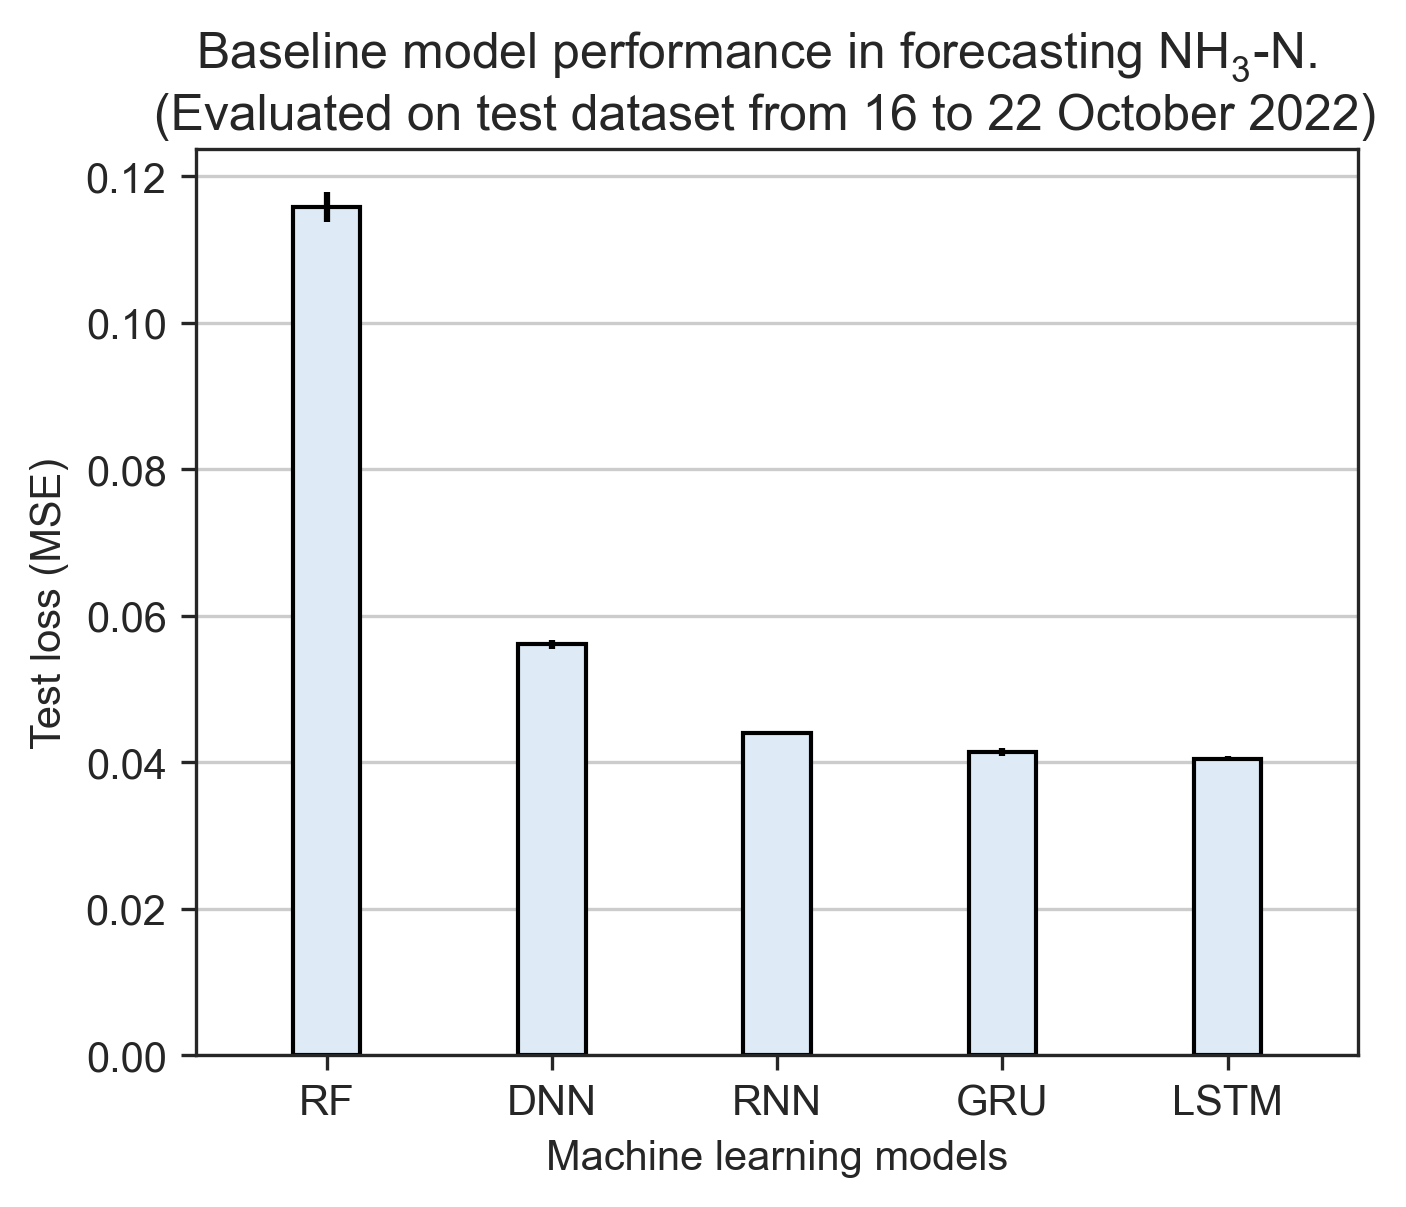
\includegraphics[width=\linewidth]{imgs/results/baseline-models-nh3.png}
      \caption{Test loss values from five ammonia forecasting models.} \label{fig:baseline-nh3}
    \end{subfigure}%
    \hspace{2em}%   % maximize separation between the subfigures
    \begin{subfigure}[t]{0.45\textwidth}
      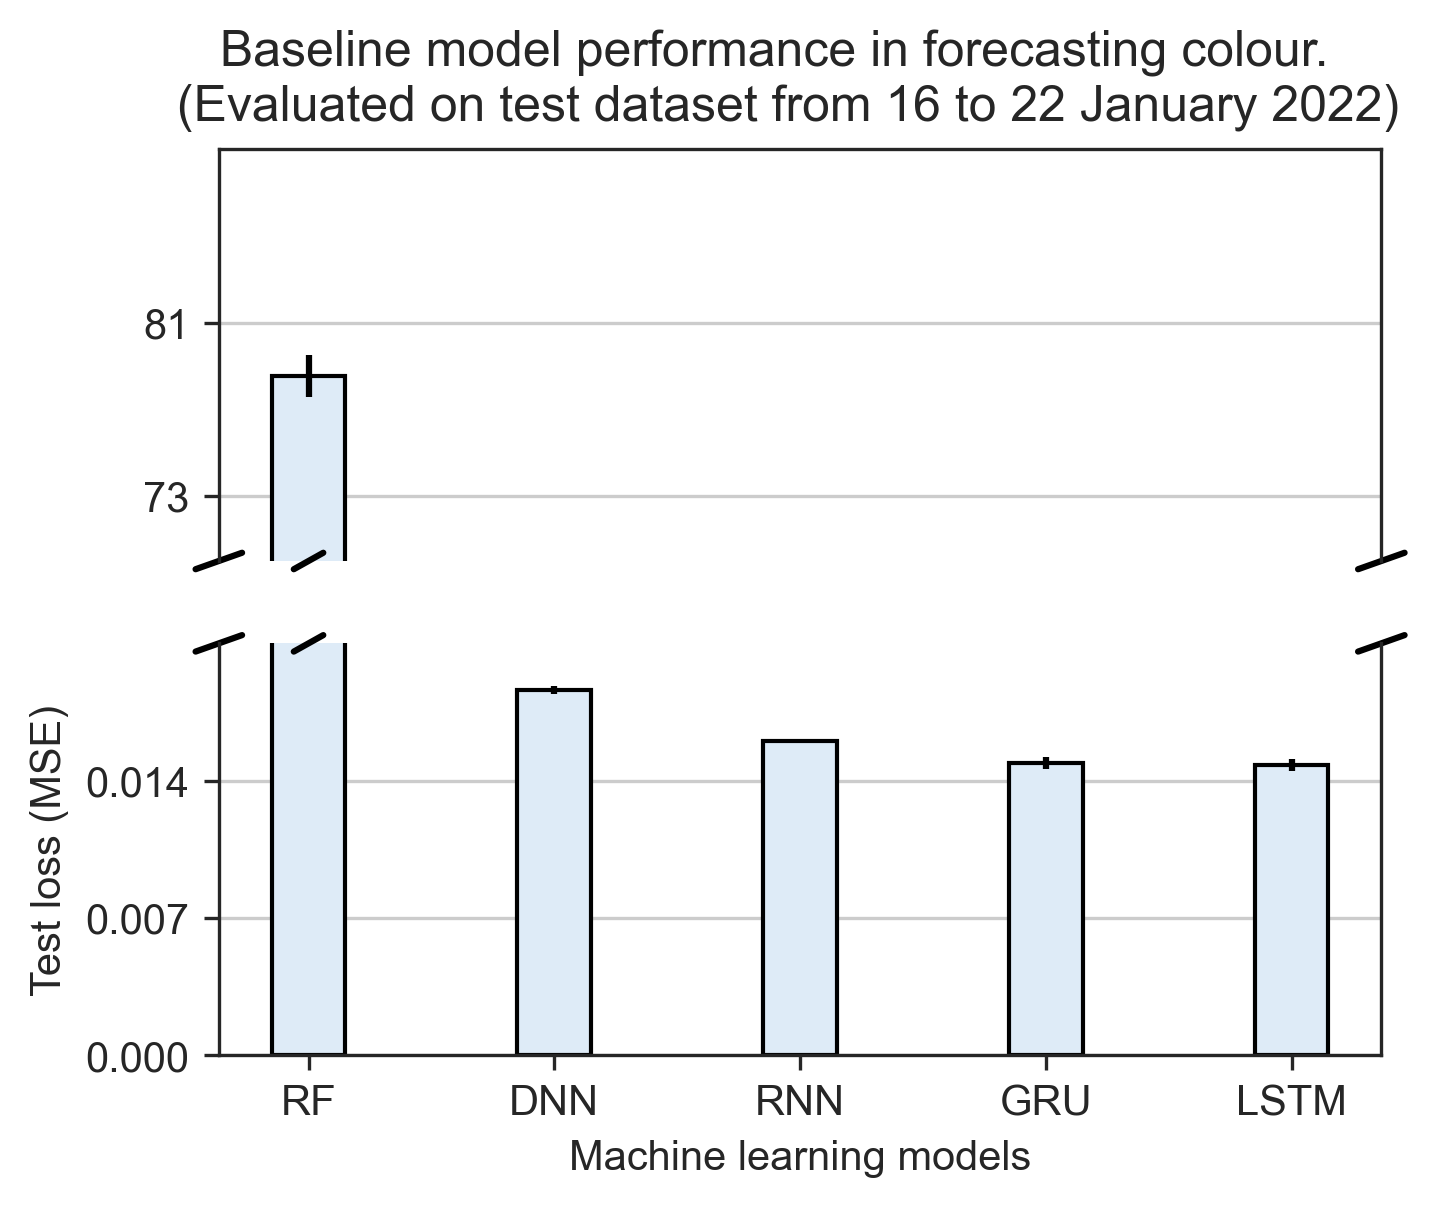
\includegraphics[width=\linewidth]{imgs/results/baseline-models-colour.png}
      \caption{Test loss values from five colour forecasting models.} \label{fig:baseline-colour}
    \end{subfigure}%  
  \caption{Baseline performance of ammonia and colour forecasting models.} \label{fig:baseline-performance}
\end{figure}


\begin{figure}[h]
    \centering
    \hspace{1em}%
    \begin{subfigure}[t]{0.45\textwidth}
      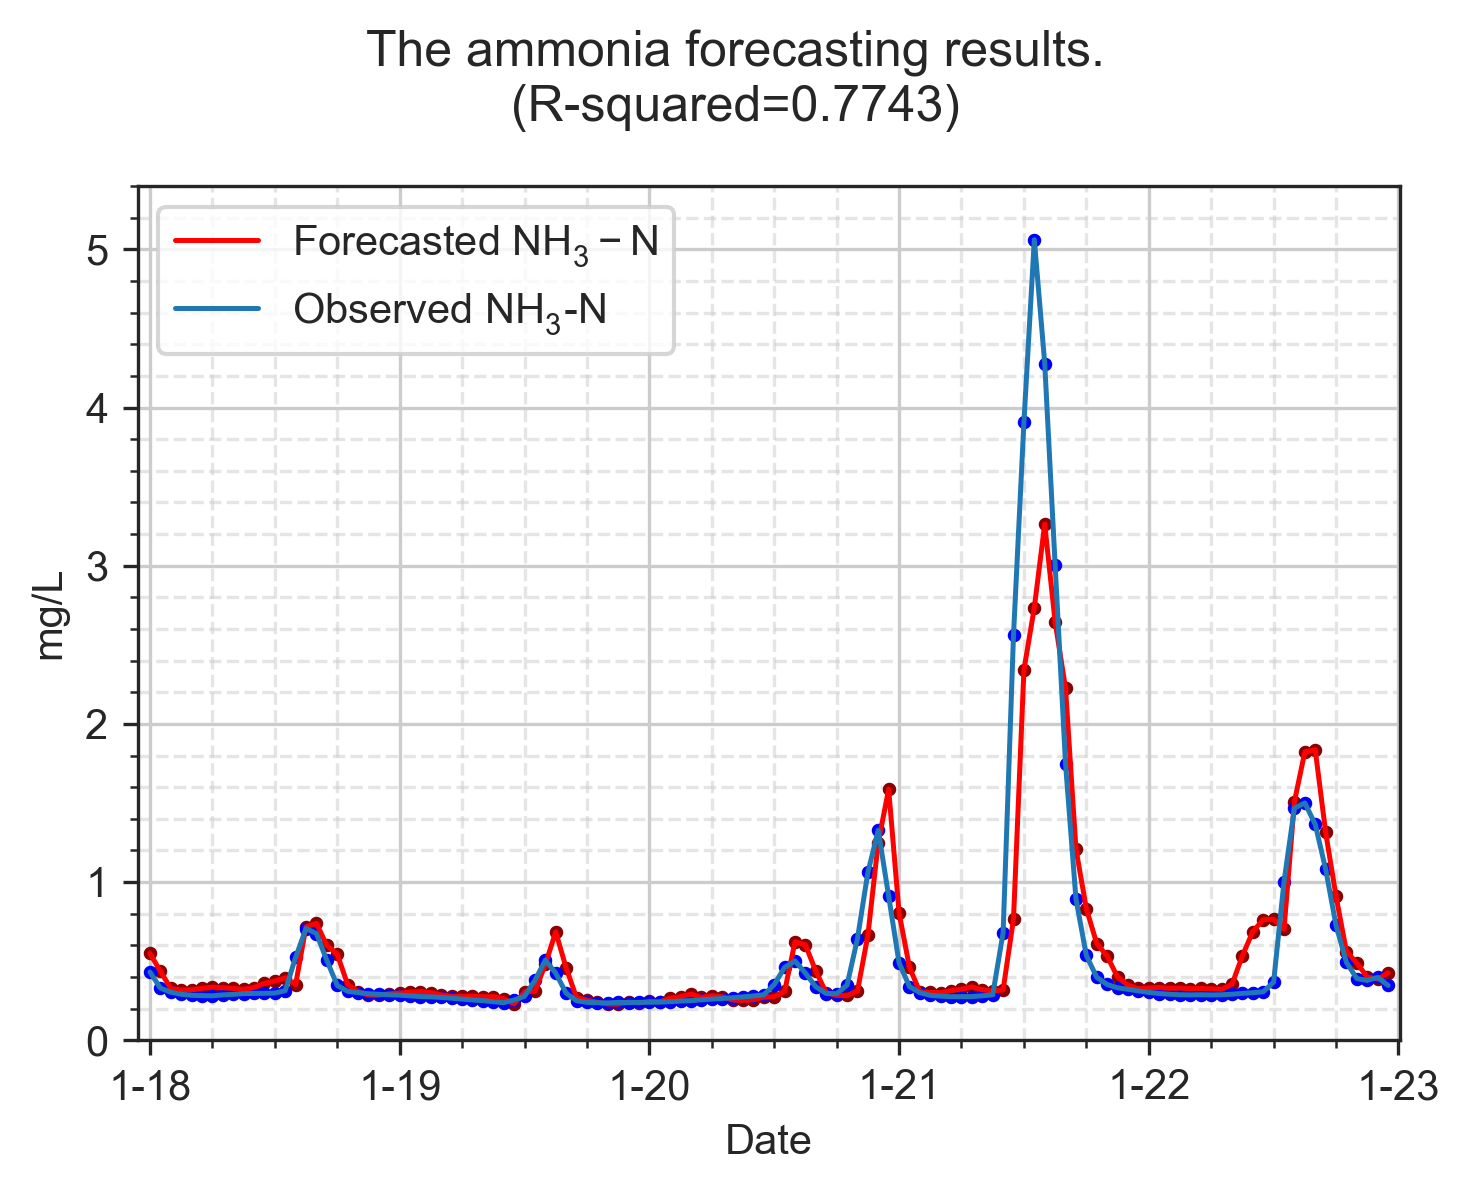
\includegraphics[width=\linewidth]{imgs/results/ammonia-colour-forecast-plot/00-RF_1_pred_Step1-obs-nh3.png}
      \caption{Baseline RF model forecasting ammonia concentration.} \label{fig:baseline-nh3-plot-rf}
    \end{subfigure}%
    \hspace{1em}%   % maximize separation between the subfigures
    \begin{subfigure}[t]{0.45\textwidth}
      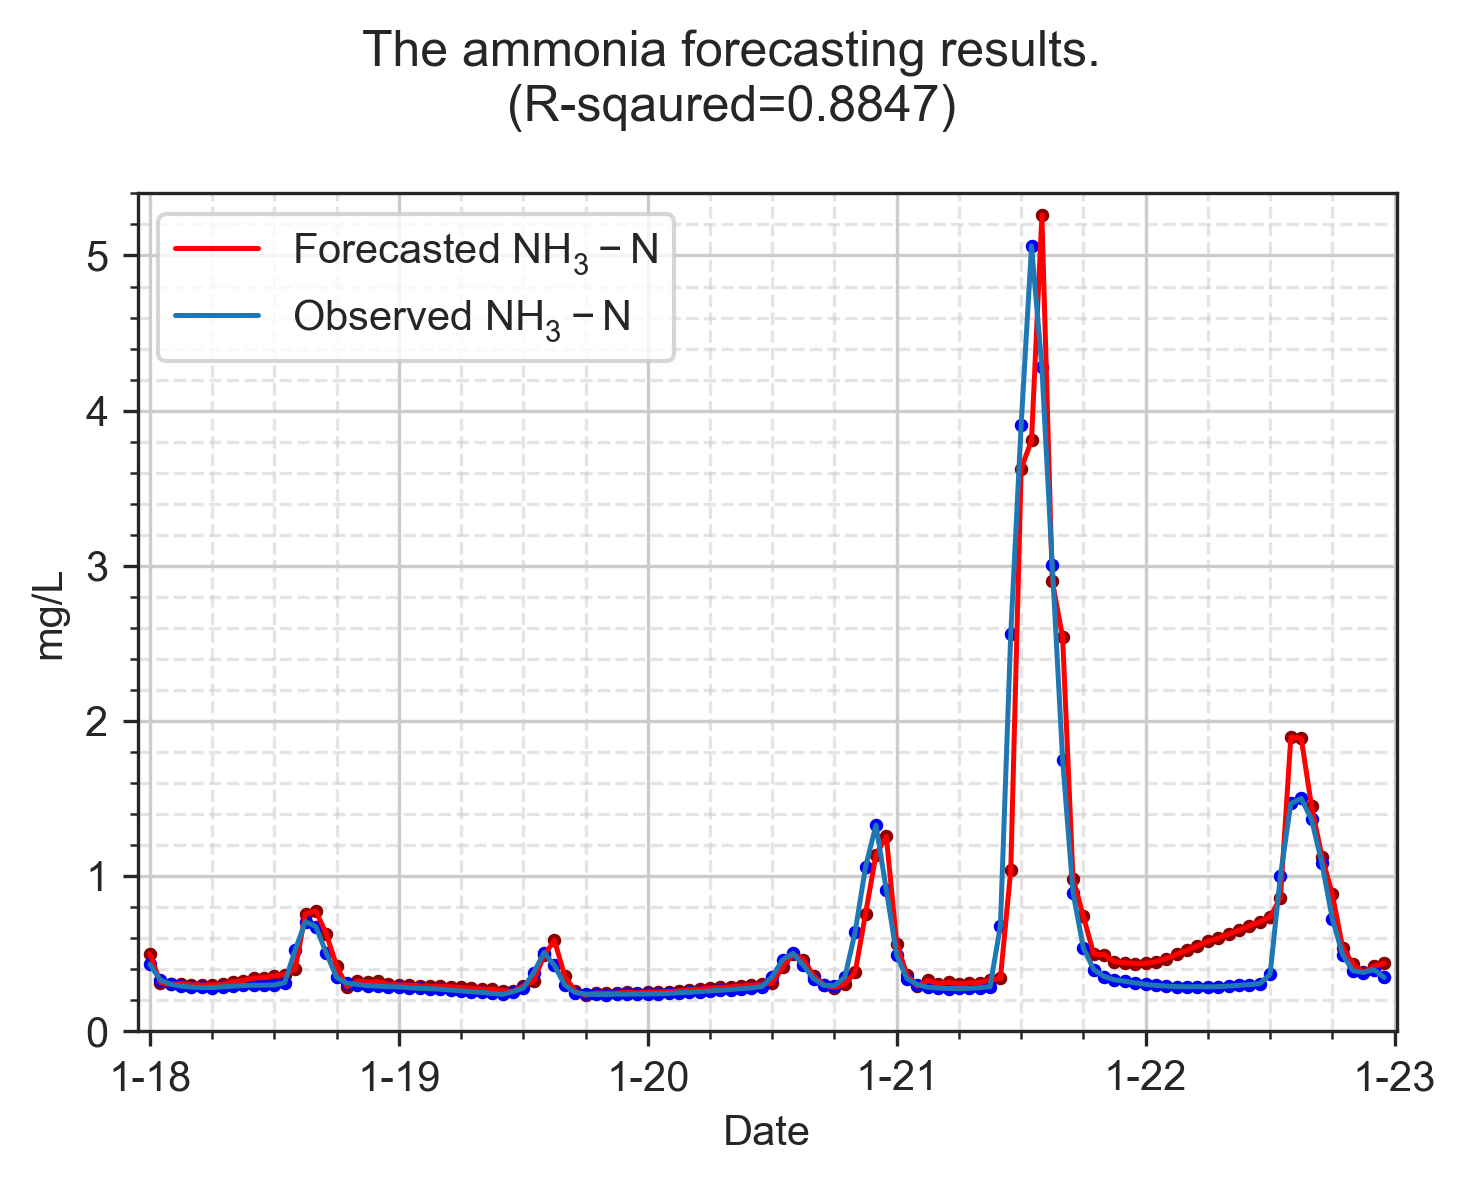
\includegraphics[width=\linewidth]{imgs/results/ammonia-colour-forecast-plot/00-LSTM_1_pred_Step1-obs-nh3.png}
      \caption{Baseline LSTM model forecasting ammonia concentration.} \label{fig:baseline-nh3-plot-lstm}
    \end{subfigure}%
    \hspace{1em}%   % maximize separation between the subfigures
    \begin{subfigure}[t]{0.45\textwidth}
      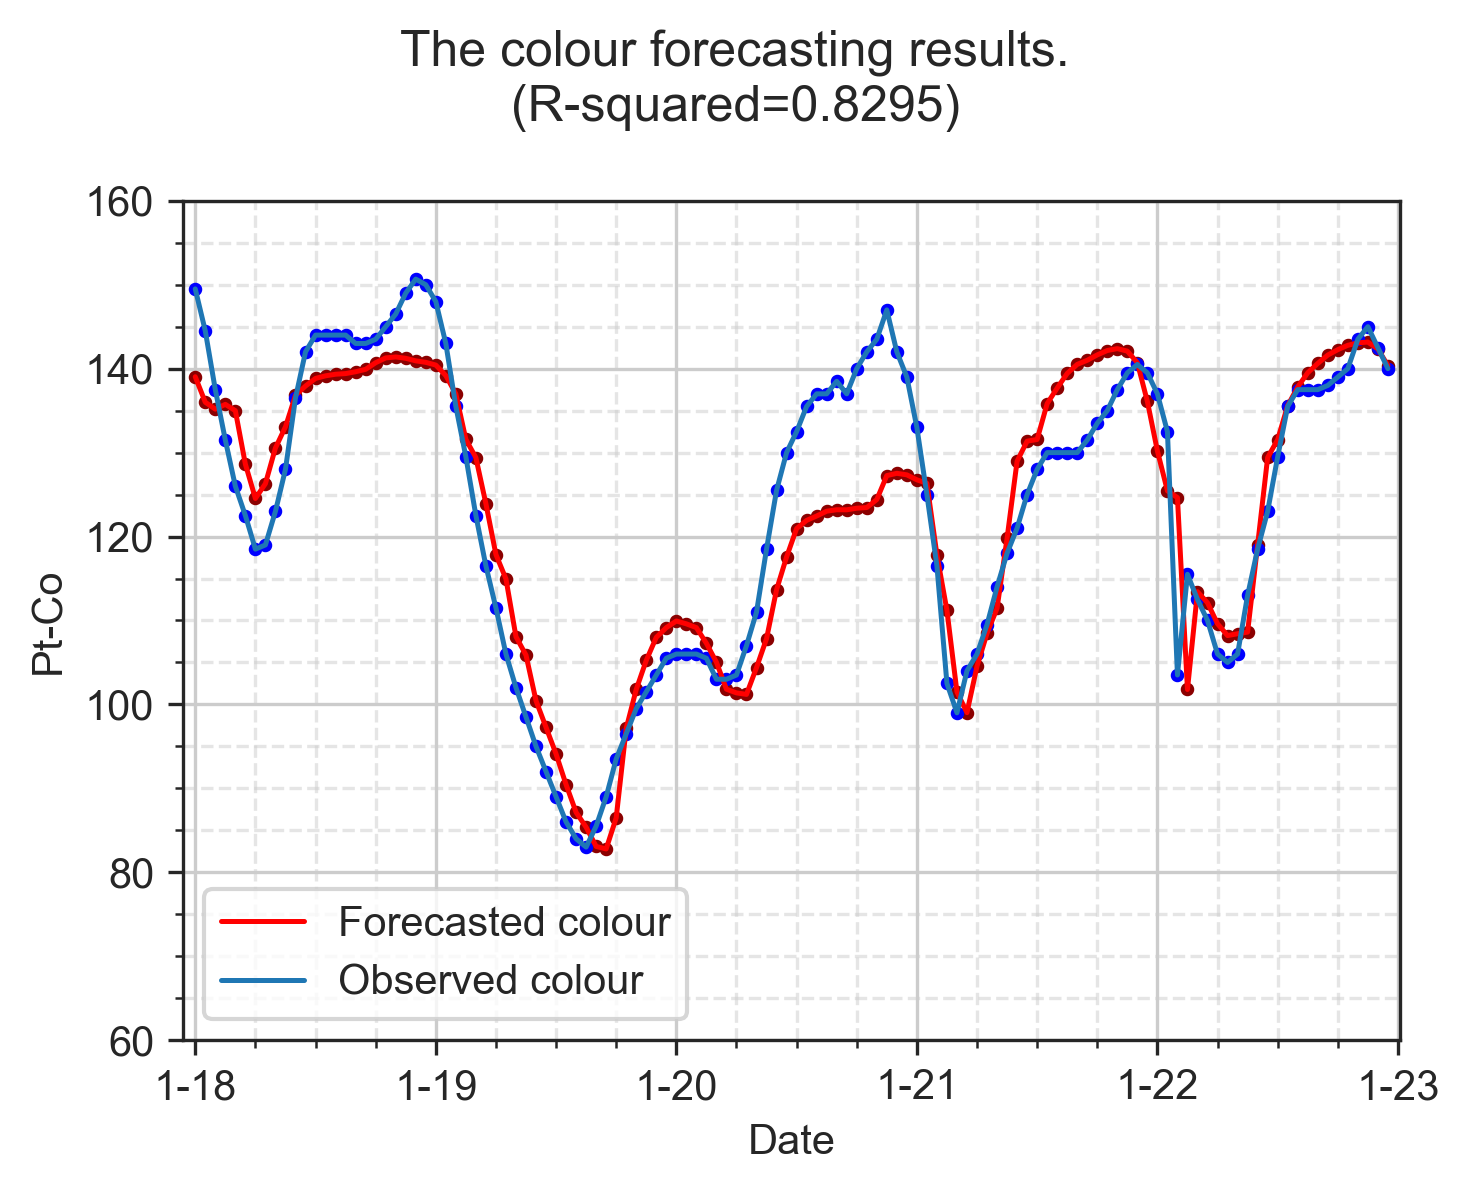
\includegraphics[width=\linewidth]{imgs/results/ammonia-colour-forecast-plot/00-RF_1_pred_Step1-obs-colour.png}
      \caption{Baseline RF model forecasting colour levels.} \label{fig:baseline-colour-plot-rf}
    \end{subfigure}% 
    \hspace{1em}%   % maximize separation between the subfigures
    \begin{subfigure}[t]{0.45\textwidth}
      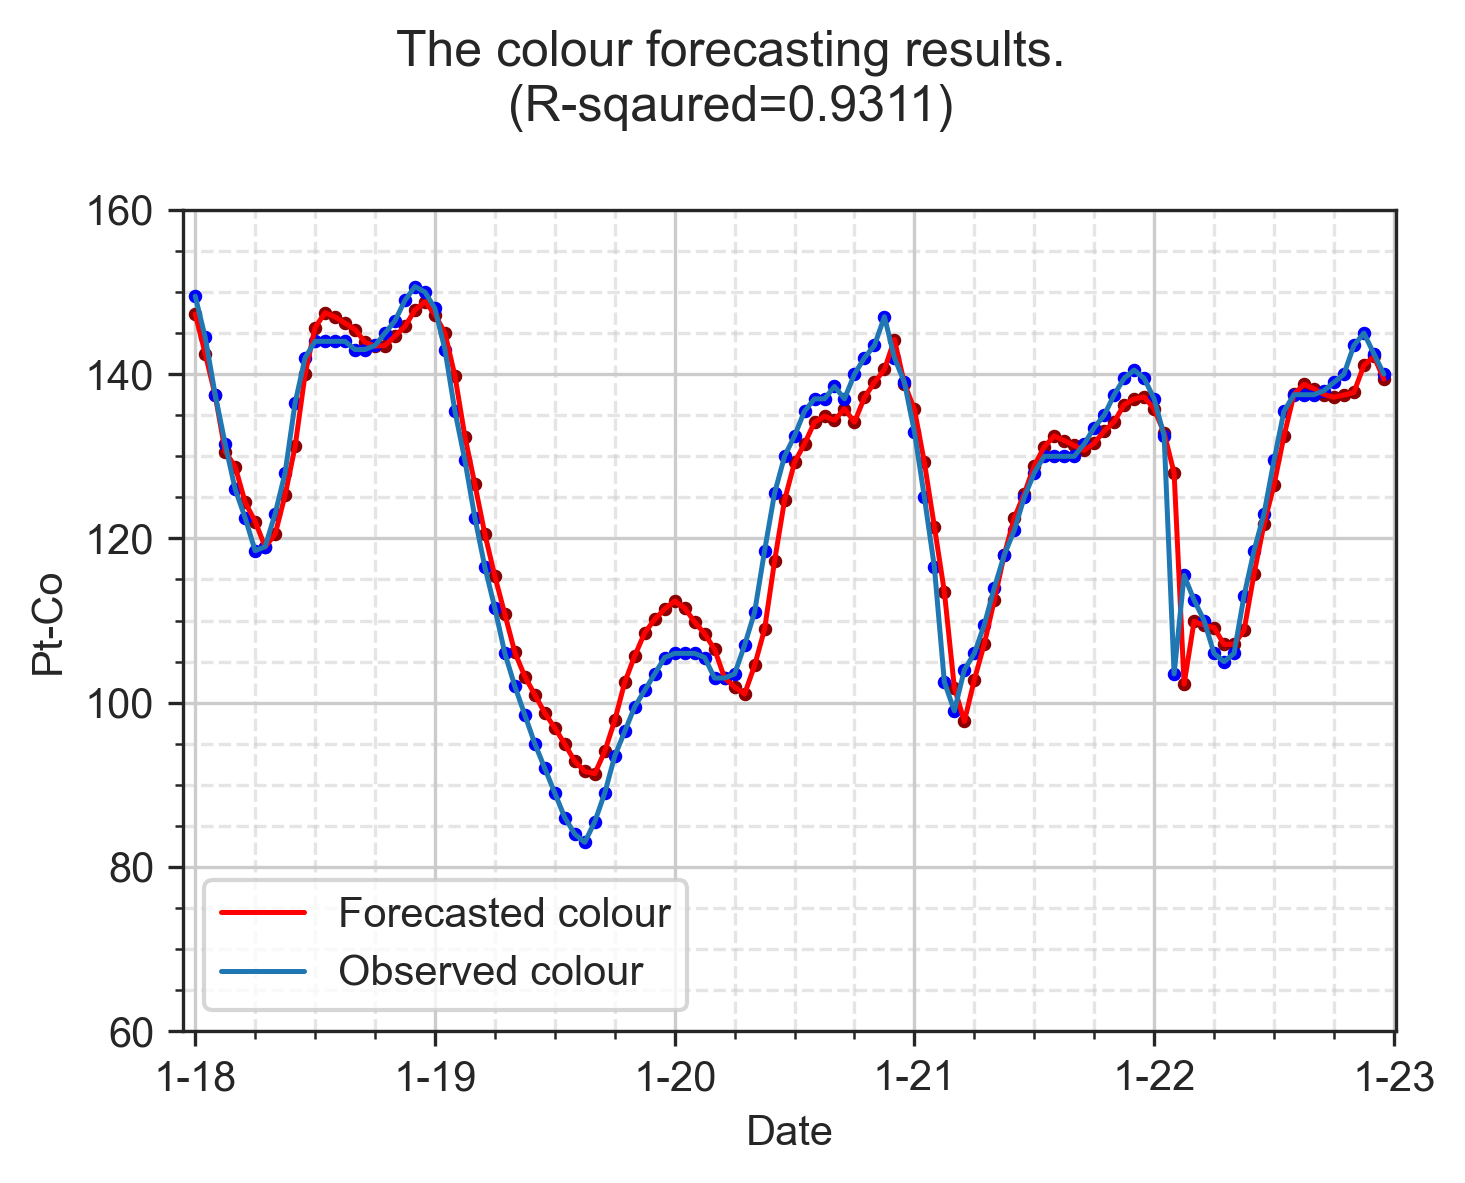
\includegraphics[width=\linewidth]{imgs/results/ammonia-colour-forecast-plot/00-LSTM_1_pred_Step1-obs-colour.png}
      \caption{Baseline LSTM model forecasting colour levels.} \label{fig:baseline-colour-plot-lstm}
    \end{subfigure}% 
  \caption{Visulization of the model forecasting results.} \label{fig:baseline-plot}
\end{figure}

RF models have the worst model performance with baseline model, even with the models trained by any of the pre-processing methods. There is a clear gap between the largest test loss values of 0.0574 from DNN-sg9 and the smallest test loss values of 0.1158 from RF models. The results highlighted the use of deep learning models have a stable and superior performance over the traditional machine learning models.

\section{Improved performance on forecasting models using data pre-processing techniques}
With the best baseline performance is known, we found that SG filters improved the quality of the raw dataset, as the top lowest test loss values are from GRU models trained by a single-feature dataset processed with SG filter at the window size of 7 and 5 (GRU-sg7 and GRU-sg5), followed by LSTM models trained by a single-feature dataset processed with EWMA filter at window size of 3 and SG filters at window size of 5 and 7. The improvements of model performance resulted from the use of data smoothing methods are not consistant across different models, in other words, the best combination of Model-Dataset to GRU model is SG filter at window size of 7, while it is EWMA at the window size of 3 for LSTM model.

Empirically, when different models are evaluated by the same testing dataset, the Model-Dataset order of test and validation loss from the smallest to largest values should be identical. However, we observed that the top three lowest validation loss values, which are 1.0796 from LSTM-ew3, 1.0969 from LSTM-ew2, and 1.1219 from LSTM-ew4, do not correspond to the Model-Dataset top three lowest test loss values. This finding points to the potential of the heterogeneity between the trianing and testing datasets. Further tests were carried out using testing dataset from October to exclude the posstibilty of having heterogeneity between the two datasets. To the best of my understanding, the comparisons between testing and validation loss are not discussed on the currently availabe research papers in modelling in wastewater treatment industry.

\begin{table}[!ht]
  \centering
  \caption{Baseline performance of ammonia forecasting model, evaluated on test dataset from \textbf{16 to 22 Janurary 2022}. Loss values are calculated by MSE.}\label{tab:baseline-result-jan-nh3}
  \begin{NiceTabular}{lcclcc}
      \toprule
      Model-Dataset & Test loss & Valid loss & Model-Dataset & Test loss & Valid loss \\
      \midrule
      GRU-sg7  & 0.0383 &1.2508&RNN-or  & 0.0432&1.6345 \\
      GRU-sg5  & 0.0385 &1.2644&RNN-ew3 & 0.0434&1.6041 \\
      LSTM-ew3 & 0.0388 &1.0796&RNN-obs & 0.0440&1.6734 \\
      LSTM-sg5 & 0.0388 &1.2346&RNN-sg9 & 0.0442&1.7046 \\
      LSTM-sg7 & 0.0388 &1.1804&DNN-obs & 0.0561&3.2383 \\
      GRU-ew2  & 0.0389 &1.1891&DNN-sg5 & 0.0562&3.2170 \\
      GRU-ew4  & 0.0391 &1.2390&DNN-ew2 & 0.0563&3.1677 \\
      GRU-ew3  & 0.0392 &1.2199&DNN-ew3 & 0.0569&3.2317 \\
      LSTM-ew2 & 0.0392 &1.0969&DNN-sg7 & 0.0570&3.2014 \\
      LSTM-ew4 & 0.0395 &1.1219&DNN-ew4 & 0.0571&3.2188 \\
      GRU-sg9  & 0.0396 &1.3097&DNN-or  & 0.0572&3.1972 \\
      LSTM-or  & 0.0398 &1.2612&DNN-sg9 & 0.0574&3.2484 \\
      LSTM-obs & 0.0405 &1.3993&RF-obs  & 0.1158&- \\
      GRU-or   & 0.0405 &1.2366&RF-sg9  & 0.1196&- \\
      LSTM-sg9 & 0.0410 &1.3076&RF-ew2  & 0.1286&- \\
      GRU-obs  & 0.0414 &1.3638&RF-or   & 0.1294&- \\
      RNN-sg5  & 0.0415 &1.5088&RF-sg5  & 0.1298&- \\
      RNN-ew2  & 0.0421 &1.5425&RF-ew3  & 0.1313&- \\
      RNN-sg7  & 0.0423 &1.6267&RF-sg7  & 0.1409&- \\
      RNN-ew4  & 0.0432 &1.5992&RF-ew4  & 0.1441&- \\
      \bottomrule
  \end{NiceTabular}
\end{table}

As shown in Table.~\ref{tab:baseline-result-oct-nh3}, the Model-Dataset ranks of top three lowest validation loss from the smallest to the largest values is identical to the ranks of the test loss values. This is in good agreement with how the heterogeneity of the datasets can impact on the model performance. The evluations of ammonia forecasting models in October 2021 showed different outcomes compared to the one in January 2022. Despite the ranks of the baseline performance remained the same, LSTM models trained by EMWA filters took the top three lowest test loss values, which are 0.0158 from LSTM-ew3, 0.0161 from LSTM-ew2 and 0.0163 from LSTM-ew4. 

\begin{table}[!ht]
    \centering
    \caption{Baseline performance of ammonia forecasting model, evaluated on test dataset from \textbf{10 to 16 October 2021}. Loss values are calculated by MSE.}\label{tab:baseline-result-oct-nh3}
    \begin{NiceTabular}{lcclcc}
        \toprule
        Model-Dataset & Test loss & Valid loss & Model-Dataset & Test loss & Valid loss \\
        \midrule
        LSTM-ew3 & 0.0158 & 1.0796 & RNN-or  & 0.0197 & 1.6345 \\
        LSTM-ew2 & 0.0161 & 1.0969 & RNN-sg7 & 0.0201 & 1.6267 \\
        LSTM-ew4 & 0.0163 & 1.1219 & RNN-sg9 & 0.0205 & 1.7046 \\
        LSTM-sg5 & 0.0166 & 1.2346 & RNN-obs & 0.0206 & 1.6734 \\
        GRU-ew3  & 0.0167 & 1.2199 & DNN-ew3 & 0.0316 & 3.2317 \\
        GRU-ew4  & 0.0169 & 1.2390 & DNN-or  & 0.0316 & 3.1972 \\
        GRU-ew2  & 0.0170 & 1.1891 & DNN-sg7 & 0.0316 & 3.2014 \\
        GRU-sg9  & 0.0174 & 1.3097 & DNN-ew2 & 0.0318 & 3.1677 \\
        LSTM-obs & 0.0175 & 1.2366 & DNN-ew4 & 0.0319 & 3.2188 \\
        LSTM-or  & 0.0177 & 1.2612 & DNN-obs & 0.0319 & 3.2383 \\
        GRU-sg5  & 0.0178 & 1.2644 & DNN-sg5 & 0.0319 & 3.2170 \\
        GRU-sg7  & 0.0180 & 1.2508 & DNN-sg9 & 0.0319 & 3.2484 \\
        LSTM-sg7 & 0.0180 & 1.1804 & RF-sg9  & 0.1307 & - \\
        GRU-or   & 0.0187 & 1.3993 & RF-sg7  & 0.1311 & - \\
        LSTM-sg9 & 0.0188 & 1.3076 & RF-sg5  & 0.1343 & - \\
        GRU-obs  & 0.0189 & 1.3638 & RF-ew2  & 0.1346 & - \\
        RNN-ew4  & 0.0190 & 1.5992 & RF-ew3  & 0.1368 & - \\
        RNN-ew2  & 0.0191 & 1.5425 & RF-obs  & 0.1443 & - \\
        RNN-ew3  & 0.0193 & 1.6041 & RF-ew4  & 0.1451 & - \\
        RNN-sg5  & 0.0195 & 1.5088 & RF-or   & 0.1477 & - \\
        \bottomrule
    \end{NiceTabular}
\end{table}

\subsection{Colour forecasting model}
In the baseline performance of colour forecasting model, LSTM-obs has the lowest test loss values of 0.0148, followed by GRU-obs, RNN-obs, DNN-obs and RF-obs, as shown in Table.~\ref{tab:baseline-result-jan-colour}. The best performed models are the LSTM models trained by EWMA filters, which are 0.0136 from LSTM-ew4, 0.0138 from LSTM-ew2 and LSTM-ew3. Interstingly, the use of LSTM models and pre-processed with EWMA filters can generate the best performed models for both the forecasting of ammonia concentration and colour levels.

\begin{table}[!ht]
  \centering
  \caption{Baseline performance of colour forecasting model, evaluated on test dataset from \textbf{16 to 22 Janurary 2022}. Loss values are calculated by MSE.}\label{tab:baseline-result-jan-colour}
  \begin{NiceTabular}{lcclcc}
      \toprule
      Model-Dataset & Test loss & Valid loss & Model-Dataset & Test loss & Valid loss \\
      \midrule
      LSTM-ew4 & 0.0136 &0.7515&RNN-obs  & 0.0160 &1.0623 \\
      LSTM-ew2 & 0.0138 &0.8011&LSTM-sg7 & 0.0161 &0.7439 \\
      LSTM-ew3 & 0.0138 &0.7547&LSTM-sg5 & 0.0168 &0.8355 \\
      GRU-ew3  & 0.0140 &0.8068&DNN-sg5  & 0.0180 &1.4702 \\
      GRU-ew2  & 0.0142 &0.8330&DNN-sg7  & 0.0180 &1.4823 \\
      GRU-ew4  & 0.0143 &0.7694&DNN-sg9  & 0.0180 &1.4574 \\
      LSTM-sg9 & 0.0143 &0.7137&DNN-ew4  & 0.0181 &1.4632 \\
      RNN-ew3  & 0.0144 &0.8492&DNN-ew3  & 0.0182 &1.4716 \\
      RNN-ew4  & 0.0147 &0.8476&DNN-ew2  & 0.0183 &1.4946 \\
      RNN-sg9  & 0.0147 &0.8363&DNN-obs  & 0.0186 &1.5397 \\
      LSTM-obs & 0.0148 &0.9744&RF-sg9   & 63.6847& \\
      GRU-obs  & 0.0149 &0.9927&RF-sg7   & 73.8263& \\
      RNN-ew2  & 0.0150 &0.9083&RF-ew3   & 75.1974&- \\
      GRU-sg9  & 0.0151 &0.7575&RF-ew4   & 77.8829&- \\
      RNN-sg5  & 0.0158 &0.8846&RF-obs   & 78.5296&- \\
      RNN-sg7  & 0.0158 &0.8755&RF-ew2   & 78.8753&- \\
      GRU-sg7  & 0.0159 &0.7791&RF-sg5   & 81.0696&- \\
      GRU-sg5  & 0.0160 &0.8080&    -    &     -  &- \\
      \bottomrule
  \end{NiceTabular}
\end{table}

From comparing the baseline performance and the influence of data smoothing methods on different models, our findings appear to be well substantiated the use of LSTM models for training ammonia and colour forecasting models due to it's outstanding model performance on test loss. The influence of pre-processing methods are not consistant on improving the model performance. Thus, datasets applied with all the pre-processing methods will be remained to test how the additional features affect the model performance.

\section{Data enrichment via feature engineering based on effluent quality pattern}



\section{Design of model architecture through analyzing wastewater composition in sewer system}
